\documentclass[12pt,a4paper]{article}
% math_setup.tex
% Essential Packages
\RequirePackage{etex}
\usepackage{comment}
\usepackage{etex}
\usepackage{listings}
\usepackage{amsmath}    % Advanced math typesetting
\usepackage{amsfonts}   % Math fonts
\usepackage{amssymb}    % Math symbols
\usepackage{amsthm}     % Theorem environment
\usepackage{mathtools}  % More symbols
\usepackage{tikz}       % For drawing diagrams
\usepackage{tikz-network}
\usepackage{pgfplots}
\usetikzlibrary{calc, arrows.meta, positioning, quotes}
\usepackage{mdframed}
\usepackage{float}
\usepackage{thmtools}
\usepackage{xcolor}
\usepackage{geometry}
\usepackage{fancyhdr}
\usepackage[colorlinks=true, linkcolor=blue, citecolor=green, urlcolor=red]{hyperref}
\usepackage{csquotes}
\usepackage[backend=biber, style=ieee]{biblatex}
\pgfplotsset{compat=1.18}
%\usepackage{mdframed}

% Wolfram Code Block
\lstdefinelanguage{Wolfram}{
    keywords={Sum, If, For, While, Do, Plot, Table, Range, Integrate, NIntegrate, D, Solve, NSolve, DSolve, NDSolve, LinearSolve, Expand, Factor, Simplify, FullSimplify, Module, Block, With},
    sensitive=true,
    morecomment=[l]{(*},
    morecomment=[s][\itshape]{(*}{*)},
    morestring=[b]",
    morestring=[b]',
}

\lstset{
    language=Wolfram,
    basicstyle=\ttfamily,
    keywordstyle=\color{blue}\bfseries,
    commentstyle=\color{green}\itshape,
    stringstyle=\color{red},
    showstringspaces=false,
    frame=single,
    breaklines=true,
    numbers=left,
    numberstyle=\tiny\color{gray},
    stepnumber=1,
    numbersep=5pt,
    backgroundcolor=\color{lightgray!20}
}

% add ref
\addbibresource{references.bib}
% Define colors
\definecolor{theoremcolor}{RGB}{230,230,250}  % Light purple
\definecolor{lemmacolor}{RGB}{240,248,255}    % Alice Blue
\definecolor{propcolor}{RGB}{240,255,240}     % Light green
\definecolor{corollarycolor}{RGB}{255,250,240} % Light orange
\definecolor{axiomcolor}{RGB}{255,240,245}    % Lavender blush
\definecolor{definitioncolor}{RGB}{240,255,255} % Light cyan
\definecolor{remarkcolor}{RGB}{245,245,245}   % Light gray
\definecolor{notationcolor}{RGB}{255,250,205}

% Boxed environments

\declaretheoremstyle[
    headfont=\normalfont\bfseries,
    bodyfont=\normalfont,
    headpunct={:},
    postheadspace=1em,
    mdframed={
        linecolor=black,
        backgroundcolor=definitioncolor,
        topline=true,
        bottomline=true,
        leftline=true,
        rightline=true,
        roundcorner=5pt
    }
]{boxeddefinitionstyle}

\declaretheorem[style=boxeddefinitionstyle, name=Definition]{definition}

\declaretheoremstyle[
    headfont=\normalfont\bfseries,
    bodyfont=\normalfont,
    headpunct={:},
    postheadspace=1em,
    mdframed={
        linecolor=black,
        backgroundcolor=theoremcolor,
        topline=true,
        bottomline=true,
        leftline=true,
        rightline=true,
        roundcorner=5pt
    }
]{boxedtheoremstyle}

% Theorem
\declaretheorem[style=boxedtheoremstyle, name=Theorem]{theorem}

% Lemma (adjust color)
\declaretheoremstyle[
    headfont=\normalfont\bfseries,
    bodyfont=\normalfont,
    headpunct={:},
    postheadspace=1em,
    mdframed={
        linecolor=black,
        backgroundcolor=lemmacolor,
        topline=true,
        bottomline=true,
        leftline=true,
        rightline=true,
        roundcorner=5pt
    }
]{boxedlemmastyle}
\declaretheorem[style=boxedlemmastyle, name=Lemma]{lemma}

% Proposition (adjust color)
\declaretheoremstyle[
    headfont=\normalfont\bfseries,
    bodyfont=\normalfont,
    headpunct={:},
    postheadspace=1em,
    mdframed={
        linecolor=black,
        backgroundcolor=propcolor,
        topline=true,
        bottomline=true,
        leftline=true,
        rightline=true,
        roundcorner=5pt
    }
]{boxedpropstyle}
\declaretheorem[style=boxedpropstyle, name=Proposition]{proposition}

% Corollary (adjust color)
\declaretheoremstyle[
    headfont=\normalfont\bfseries,
    bodyfont=\normalfont,
    headpunct={:},
    postheadspace=1em,
    mdframed={
        linecolor=black,
        backgroundcolor=corollarycolor,
        topline=true,
        bottomline=true,
        leftline=true,
        rightline=true,
        roundcorner=5pt
    }
]{boxedcorollarystyle}
\declaretheorem[style=boxedcorollarystyle, name=Corollary]{corollary}

% Axiom (boxed)
\declaretheoremstyle[
    headfont=\normalfont\bfseries,
    bodyfont=\normalfont,
    headpunct={:},
    postheadspace=1em,
    mdframed={
        linecolor=black,
        backgroundcolor=axiomcolor,
        topline=true,
        bottomline=true,
        leftline=true,
        rightline=true,
        roundcorner=5pt
    }
]{boxedaxiomstyle}
\declaretheorem[style=boxedaxiomstyle, name=Axiom]{axiom}

% Remark environment
\declaretheoremstyle[
    headfont=\normalfont\bfseries,
    bodyfont=\normalfont,
    headpunct={:},
    postheadspace=1em,
    mdframed={
        linecolor=black,
        backgroundcolor=remarkcolor,
        topline=true,
        bottomline=true,
        leftline=true,
        rightline=true,
        roundcorner=5pt
    }
]{remarkstyle}
\declaretheorem[style=remarkstyle, name=Remark, numbered=no]{remark}
% Normal, non-italic environments
\declaretheoremstyle[
    headfont=\normalfont\bfseries,
    bodyfont=\normalfont,
    headpunct={:},
    postheadspace=1em,
]{normalstyle}

% Notation environment
\declaretheoremstyle[
    headfont=\normalfont\bfseries,
    bodyfont=\normalfont,
    headpunct={:},
    postheadspace=1em,
    mdframed={
        linecolor=black,
        backgroundcolor=notationcolor,
        topline=true,
        bottomline=true,
        leftline=true,
        rightline=true,
        roundcorner=5pt
    }
]{boxednotationstyle}
\declaretheorem[style=boxednotationstyle, name=Notation]{notation}


% Note environment (more noticeable, with separators, no background, no end symbol)
\newenvironment{note}[1][]
    {\par\vspace{0.5em}\noindent\rule{\textwidth}{0.4pt}\par\vspace{0.5em}%
    \textbf{Note\if\relax\detokenize{#1}\relax\else: #1\fi}\par}
    {\par\vspace{0.5em}\noindent\rule{\textwidth}{0.4pt}\par\vspace{0.5em}}

\declaretheorem[style=normalstyle, name=Note, numbered=no]{oldnote}

\declaretheorem[style=normalstyle, name=Example]{example}
\declaretheorem[style=normalstyle, name=Exercise]{exercise}
\declaretheorem[style=normalstyle, name=Statement]{statement}
\declaretheorem[style=normalstyle, name=Solution, numbered=no]{solution}

% Proof environment (normal, non-italic, with QED symbol)
\declaretheoremstyle[
    headfont=\normalfont\bfseries,
    bodyfont=\normalfont,
    headpunct={:},
    postheadspace=1em,
    qed=$\blacksquare$
]{proofstyle}

\declaretheorem[style=proofstyle, name=Proof]{customproof}

% Shorthand
\newcommand{\vect}[1]{\mathbf{#1}} % For regular vectors
\newcommand{\uvec}[1]{\hat{\mathbf{#1}}} % For unit vectors
\newcommand{\prob}[1]{
    \section*{Problem #1}
}
\newcommand{\R}{\mathbb{R}} % Real numbers
\newcommand{\Z}{\mathbb{Z}} % Integers
\newcommand{\C}{\mathbb{C}} % Complex numbers
\newcommand{\N}{\mathbb{N}} % Natural numbers
\newcommand{\Q}{\mathbb{Q}} % Rational numbers
\newcommand{\Hq}{\mathbb{H}} % Quaternions
\newcommand{\F}{\mathbb{F}} % Finite fields
\newcommand{\Proj}{\mathbb{P}} % Projective space
\newcommand{\K}{\mathbb{K}} % Arbitrary field
\newcommand{\T}{\mathbb{T}} % Torus or sometimes denoted for Topological space
\newcommand{\A}{\mathbb{A}} % Affine space
\newcommand{\0}{\mathbf{0}} % Zero vector
\newcommand{\mbf}[1]{\mathbf{#1}} 
\newcommand{\mat}[1]{\mathbf{#1}}
\newcommand{\adj}{\operatorname{adj}}
\newcommand{\dom}[1]{
    \operatorname{dom}(#1)
}




% Layout
\geometry{a4paper, margin=1in}
\pagestyle{fancy}
\fancyhf{}
\rhead{\today}
\lhead{\textbf{ENG1005 Engineering Mathematics}}
\rfoot{Page \thepage}


\begin{document}

\newcommand{\df}[2]{
    \frac{d#1}{d#2}
}

\title{ENG1005 Week8 Workshop Problem Set Solutions}
\author{Yang Xingyu (33533563)}
\date{\today}
\maketitle

\section*{Question 1}
\begin{solution}
    This differential equation is linear. Because all occurrences of $I$ and it's differentiation with respect to $t$ are linear.
\end{solution}

\begin{remark}
    Rigorously, we can identify this with the definition of \textbf{linear ODE}.
    \begin{definition}[Linear ODE]
    An ordinary differential equation of order $n$, say, is said to be linear if it assumes the general form
$$
a_0(x) \frac{d^n y}{d x^n}+a_1(x) \frac{d^{n-1} y}{d x^{n-1}}+\cdots+a_{n-1}(x) \frac{d y}{d x}+a_n(x) y=b(x)
$$

where $a_0(x) \neq 0$ and the following conditions are satisfied :
\begin{enumerate}
    \item The highest possible degree of $y$ and its derivatives is unity.
    \item Products of $y$ and any of its derivatives do not appear in equation.
    \item No term involving transcendental functions of $y$ or its derivatives is included.
\end{enumerate}
\end{definition}

We now check whether $L I^{\prime}(t)+R I(t)=E(t)$ is a first-order linear ODE, where $L$ and $R$ are constants, and $I(t)$ is either an exponential function or trigonometric function, and $E(t)$ either constant or trigonometric function, in terms of $t$, depending on AC or DC.
\begin{itemize}
    \item The degree of $\df{I}{t}$ and $I(t)$ are both one.
    \item $\df{I}{t}$ and $I(t)$ are multiplied only by a scalar, or constant coefficient in $\R$.
    \item There are no any functions in the differential equation that is dependent to $I$, and all the functions (though possibly transcendental), are all related only to $t$.
\end{itemize}
Hence, $L I^{\prime}(t)+R I(t)=E(t)$ is a first-order linear ODE.
\end{remark}

\section*{Question 2}
\begin{solution}
    When $t \geq 0$, $E(t) = 0$, hence,
$$    \begin{aligned}
LI^\prime ( t) +RI & =0\\
L\frac{dI}{dt} & =-RI\\
\frac{dI}{dt} & =I( t) \cdot \left( -\frac{R}{L}\right)
\end{aligned}$$
where$ \left( -\frac{R}{L}\right)$ is a constant function, we can define $h(t) := \left(-\frac{R}{L}\right)$.

So we get the separable form
\begin{equation} \label{W8:sep}
    \frac{dI}{dt} = I(t)h(t).
\end{equation}


To conclude, in this case, the differential equation must be separable.

\begin{remark}
Before solving the equation, we first examine its solvability by bringing forward the solvable condition of all linear ODEs.

In most cases, it is sure that an n-order linear ODE is solvable (has at least one solution).

\begin{theorem}[Existence of Solutions for Linear ODE]
Consider an \(n\)-th order linear differential equation:
\[
L(y) = a_n(x) \frac{d^n y}{dx^n} + a_{n-1}(x) \frac{d^{n-1} y}{dx^{n-1}} + \cdots + a_1(x) \frac{dy}{dx} + a_0(x) y = f(x),
\]
where \(f(x)\) is a given function and \(a_0(x), a_1(x), \dots, a_n(x)\) are the coefficient functions.

If the right-hand side \(f(x)\) is a continuous function in some interval \([a,b]\), and the coefficient functions \(a_0(x), a_1(x), \dots, a_n(x)\) are also continuous on this interval, then a solution to the differential equation \textit{exists} on this interval.

This implies that regardless of the specific form of \(f(x)\), as long as it is continuous (even only continuous in [$a,b$]), and the coefficients are continuous as well, we can guarantee the existence of a solution in a certain interval.
\end{theorem}
In general, for ordinary differential equations, \textit{continuity} is more fundamental than \textit{differentiability}. If \(f(x)\) and the coefficient functions are continuous, then a solution exists. If \(f(x)\) and the coefficients are differentiable, then the solution may be smoother (i.e., higher-order derivatives exist), but the existence of the solution only requires continuity.

We can show this with Existence-Uniqueness Theorem when discuss the existence of solutions to linear ODEs later.

Now we discuss the existence and uniqueness of the particular solution to linear ODEs. First, it is pretty clear that, without extra \textbf{valid} information provided as in IVP or BVP, we can only get a general solution that contains a constant term $C$, which can be taken as a subset of $\mathbf{C}^n(\R)$: the set of all real functions that are n-th order differentiable.

When it comes to the existence of a distinct, particular solution, we may refer to Existence and Uniqueness Theorem \parencite{dey_differential_2021}.

\begin{theorem}[Existence-Uniqueness Theorem (Picard-Lindelöf)]
Let $\frac{dy}{dx} = f(x, y)$
be an ODE subject to the initial condition \( y(x_0) = y_0 \).

If:

(a) \( f(x, y) \) is continuous for every \( (x, y) \in D \), where \( D \) is a rectangle bounded by the straight lines \( x = x_0 \pm a \) and \( y = y_0 \pm b \) in \( \mathbb{R} \).

(b) \( f(x, y) \) satisfies the Lipschitz condition of order 1, namely:
\[
|f(x, y_1) - f(x, y_2)| \leq K |y_1 - y_2|,
\]
where \( K \) is a constant dependent on \( D \), then there exists a unique solution \( y = \bar{y}(x) \) to the ODE such that \( y_0 = \bar{y}(x_0) \) for all \( x \in [x_0 - \delta, x_0 + \delta] \), where
\[
\delta < \min \left\{ a, \frac{b}{M}, \frac{1}{K} \right\} \quad \text{and} \quad M = \max_{(x, y) \in D} f(x, y).
\]
\end{theorem}
\begin{note}
    The proof the the theorem is not compulsory to most people, and may take some time to show the technique applied (Picard iteration), but you may find it \href{https://en.wikipedia.org/wiki/Picard%E2%80%93Lindel%C3%B6f_theorem}{here} in case that you already have some basics of real analysis.
\end{note}
     We also show how can we derive Lipschitz Continuity from the general definition to continuity in function. For consistency with the theorem, we will give the definition in binary functions.
\begin{definition}[Continuity]
    A function \( f(x, y) \) is continuous at \( (x_0, y_0) \) if for any \( \varepsilon > 0 \), there exists \( \delta > 0 \) such that:
\[
|(x, y) - (x_0, y_0)| < \delta \quad \implies \quad |f(x, y) - f(x_0, y_0)| < \varepsilon.
\]
This ensures small changes in \( (x, y) \) produce small changes in \( f(x, y) \).
\end{definition}
Lipschitz continuity is a stricter condition. A function is Lipschitz continuous in \( y \) if there exists \( K > 0 \) such that for any \( x \in D \) and all \( y_1, y_2 \in D \),
\[
|f(x, y_1) - f(x, y_2)| \leq K |y_1 - y_2|.
\]
While continuity guarantees no jumps, Lipschitz continuity controls the rate of change, bounding it by \( K \).

Lipschitz continuity implies continuity: given \( f(x, y) \) Lipschitz continuous, for any \( y_1, y_2 \),
\[
|f(x, y_1) - f(x, y_2)| \leq K |y_1 - y_2|.
\]
By setting \( \delta = \frac{\varepsilon}{K} \), if \( |y_1 - y_2| < \delta \), then \( |f(x, y_1) - f(x, y_2)| < \varepsilon \), which satisfies the continuity condition. Thus, every Lipschitz continuous function is continuous, but not every continuous function is Lipschitz, as general continuity lacks a bound on the rate of change.

There are more worth discussing on Lipschitz condition, since in real practice, we tend to use it's equivalent condition, which is easier to prove. 
\begin{corollary}
    For functions that are differentiable with respect to \( y \), the Lipschitz condition can be equivalently expressed in terms of the partial derivative. If the partial derivative of \( f(x, y) \) with respect to \( y \) is bounded, i.e.,
\[
\left| \frac{\partial f(x, y)}{\partial y} \right| \leq K \quad \text{for all } (x, y) \in D,
\]
then the function is Lipschitz continuous with respect to \( y \). In this case, the Lipschitz constant \( K \) is exactly the upper bound on the partial derivative.
\end{corollary}
\begin{proof}
To prove that bounded partial derivatives imply Lipschitz continuity, we proceed as follows:

\begin{enumerate}
    \item Assume that \( f(x, y) \) is continuously differentiable with respect to \( y \). Then for any two points \( y_1 \) and \( y_2 \), the fundamental theorem of calculus gives:
\[
f(x, y_1) - f(x, y_2) = \int_{y_2}^{y_1} \frac{\partial f(x, t)}{\partial y} \, dt
\]
    \item Taking the absolute value and applying the boundedness condition \( \left| \frac{\partial f(x, y)}{\partial y} \right| \leq K \), we have:
\[
|f(x, y_1) - f(x, y_2)| \leq \int_{y_2}^{y_1} \left| \frac{\partial f(x, t)}{\partial y} \right| \, dt \leq K |y_1 - y_2|
\]
\end{enumerate}

This confirms that if the partial derivative is bounded, the function satisfies the Lipschitz condition.
\end{proof}
 Thus, Lipschitz continuity can be viewed as an extension of the concept of bounded derivatives, guaranteeing controlled changes in the function's output as \( y \) varies.
\end{remark}
\end{solution}


\section*{Question 3}
\begin{solution}
Rearrange the equation by separating the variable, we have
\[
\frac{1}{I}dI = -\frac{R}{L}dt
\]
Integrate both sides:
\begin{align*}
\int \frac{1}{I} dI & =\int -\frac{R}{L} dt\\
\ln |I| & =-\frac{R}{L} t + C\\
I(t) & =e^{-\frac{R}{L} t + C} = Ae^{-\frac{R}{L} t},
\end{align*}
where $A := e^C$ is some constant.

\begin{remark}
The equality still holds after integrating both side.

First considering the example of two differentiable functions: $F(y)$ and $G(x)$ such that $y$ is a function with respect to $x$, and 
\begin{equation}
\label{w8:asump1}
F(y) = G(x) + C
\end{equation}


Differentiate both sides with respect to $x$:
\[
\frac{d F(y)}{d x}=\frac{d G(x)}{d x}
\]

Since $y$ itself is a relation on $x$, so by inverse chain rule, we have
\[
\frac{d F(y)}{d y} \cdot \frac{d y}{d x}=G^{\prime}(x)
\iff
F^{\prime}(y) \frac{d y}{d x}=G^{\prime}(x),
\]
which can be rearranged easily to the form of separable equation as in (\ref{W8:sep}).

This can be served as the necessary condition for the validity of integrating both sides, and now we proceed to show the sufficient condition.
\begin{proof}
    We assume $$\exists y=y(x),\text{ } \df{y}{x}=f(x)g(x).$$

    Dividing both sides by $g(x)$:
    \[
    \frac{1}{g(y)} \frac{d y}{d x}=f(x)
    \]
    Now the LHS is a product of two functions, which can be evaluated to a new function with respect to $x$ (as $y$ can be interpreted by $x$) and RHS is also a function on $x$, so, this allows us to integrate both sides to $x$ legitimately.
    \[
    \int \frac{1}{g(y)} \frac{d y}{d x} d x= \int \frac{1}{g(y)} dy= \int f(x) d x
    \]

    But this is not correct though, we need to add some constant terms to both side to keep the balance, as we cannot find exact original functions.
    \[
    \int \frac{1}{g(y)} dy + C_1 = \int f(x) d x + C_2
    \]
    Since these constants can be moved to either side, so by convention, we have
    \[
    \int \frac{1}{g(y)} dy = \int f(x) d x + C,
    \]
    which is equivalent to (\ref{w8:asump1}).
\end{proof}

Hence, we have 
\[
\df{y}{x} = f(y)g(x) \iff \int \frac{1}{g(y)} dy = \int f(x) d x + C.
\]


\end{remark}

Substitute $\begin{cases}
L=7\\R=33\\t=0.1
\end{cases}$, we have $I(0.1) = Ae^{-\frac{33}{7}\times 0.1} \approx 0.624A $

With the initial condition $I(0) = 5$, we have $A = 5$.

Therefore, $I(0.1) \approx 0.624\times 5 \approx 3.12$
\end{solution}

\section*{Question 4}
\begin{solution}
We assume that it takes $\displaystyle t_{1}$ second(s) to decay to 0.8 times of the initial value, $\displaystyle I_{0}$. We have:
\begin{gather*}
\begin{cases}
I( t_{1}) =0.8I_{0}  \\
I(0) = I_0\\
I( t_{1}) \ =\ I_{0} e^{-\frac{R}{L} t_{1}} 
\end{cases} \Longrightarrow \ln 0.8={-\frac{R}{L} t_{1}}.
\end{gather*}
Similarly,
\begin{equation*}
I( t_{1} +0.15) =0.38I_{0} = I_0 e^{^{-\frac{R}{L}( t_{1} +0.15)}} 
\implies \ln0.38 = -\frac{R}{L}( t_{1} +0.15).
\end{equation*}
These give
\[
\begin{cases}
\frac{R}{L} t_{1} \approx 0.223 & \\
\frac{R}{L}( t_{1} +0.15) \approx 0.967 & 
\end{cases}
\]

Dividing row 2 by row 1,
\[
\frac{t_{1} +0.15}{t_1} \approx \frac{0.967}{0.223} \implies t_1 \approx \frac{0.15}{3.336} \approx0.045.
\]

Hence, it takes around 0.045 second to decay to 80\% of the initial value.
\end{solution}

\section*{Question 5}
\begin{solution}
Substituting, we have
\[
5\frac{dI}{dt} +25I=150e^{-10t}\cos( 40t).
\]

Simplifying:
\[
\frac{dI}{dt} +5I=30e^{-10t}\cos( 40t).
\]

This is a Linear non-homogeneous inseparable ODE with constant coefficient, so we can either solve it using integration factor or linearity of the general solution space that $y=y_h+y_p$, i.e., undetermined coefficient method. 
\end{solution}

\section*{Question 6}
\begin{solution}
\end{solution}
We will solve
\begin{equation}\label{w8:eq}
    \frac{dI}{dt} +5I=30e^{-10t}\cos( 40t).
\end{equation}
\subsubsection*{Integration Factors}
Following the form of IF, we have
\[
\begin{cases}
    \mathcal{I}(t) = e^{\int p(t)dt}\\
    I(t) = \frac{1}{\mathcal{I}(t)} \int \mathcal{I}(t)q(t)dt + C
\end{cases}
\]
where
\begin{itemize}
    \item $\mathcal{I}(t)$ is the integration factor.
    \item $p(t) = 5$, $q(t) = 30e^{-10t}\cos(40t)$
    \item $I(t)$ is the subject of the ODE
\end{itemize}
We first evaluate the integration factor $\mathcal{I}(t)$.
\[
\mathcal{I}(t) = e^{\int 5dt} = e^{5t}
\]
Now we evaluate the solution $I(t)$:
$$\begin{aligned}
    I(t) &= e^{-5t}\int e^{5t}30e^{-10t}\cos(40t) dt + C\\
    I(t) &= e^{-5t}\int 30e^{-5t}\cos(40t) dt + C\\
\end{aligned}$$
Integrating by parts:
\[
\int 30e^{-5t}\cos(40t) dt = -\frac{6}{65} e^{-5 t}(\cos (40 t)-8 \sin (40 t)) + C
\]
So,
\[
I(t) = -\frac{6}{65} e^{-10 t}[8 \sin (40 t)-\cos (40 t)]+A e^{-5 t}
\]

By the initial condition $I(0) = 5$,
\[
I(0) = A-\frac{6}{65} = 5\implies A = \frac{331}{65} 
\]

Hence,
\begin{equation}\label{w8:conc1}
I(t) = \frac{331}{65} e^{-5 t}+ \frac{6}{65} e^{-10 t}[8 \sin (40 t)-\cos (40 t)]
\end{equation}

\begin{remark}
All first-order linear inseparable non-homogeneous ODE IVP is solvable, and has specific solution. 

\begin{theorem}[Solution of First-Order Linear Non-Homogeneous ODE]
Consider the first-order linear non-homogeneous ordinary differential equation:
\[
\frac{dy}{dx} + p(x)y = q(x)
\]
where $p(x)$ and $q(x)$ are continuous functions on an interval $I$. The general solution to this equation is given by:
\[
y(x) = \frac{1}{I(x)}\left[\int I(x)q(x)dx + C\right]
\]
where $I(x) = e^{\int p(x)dx}$ is an integrating factor, and $C$ is an arbitrary constant.
\end{theorem}

\begin{proof}
To solve this differential equation, we employ the method of integrating factors. Our goal is to find a function $I(x)$ such that when we multiply both sides of the equation by $I(x)$, the left-hand side becomes the derivative of a product.

We begin by multiplying both sides of the equation by an as-yet-undetermined function $I(x)$:

\[
I(x)\frac{dy}{dx} + I(x)p(x)y = I(x)q(x)
\]

Now, we aim to choose $I(x)$ such that the left-hand side is the derivative of the product $I(x)y$. Expanding this derivative using the product rule, we get:

\[
\frac{d}{dx}(I(x)y) = I(x)\frac{dy}{dx} + y\frac{dI}{dx}
\]

Comparing this with the left-hand side of our equation, we see that we need:

\[
y\frac{dI}{dx} = I(x)p(x)y
\]

This equality should hold for all $y$, so we can conclude:

\[
\frac{dI}{dx} = I(x)p(x)
\]

This is a separable differential equation for $I(x)$. Solving it, we find:

\[
I(x) = e^{\int p(x)dx}
\]

This is our integrating factor. With this choice of $I(x)$, our original equation becomes:

\[
\frac{d}{dx}(I(x)y) = I(x)q(x)
\]

We can now integrate both sides:

\[
I(x)y = \int I(x)q(x)dx + C
\]

where $C$ is an arbitrary constant of integration. Finally, solving for $y$, we obtain our general solution:

\[
y(x) = \frac{1}{I(x)}\left[\int I(x)q(x)dx + C\right]
\]

This completes our proof.
\end{proof}
\end{remark}
\subsubsection*{Method of Undetermined Coefficients}
We will find the solution by using the fact that any general solution is a linear combination of homogeneous solution and a particular solution:
\begin{equation}\label{w8:homo}
y = y_h+y_p.
\end{equation}

\begin{remark}
We can fully explain how this works by analysing the solution space of non-homogeneous linear ODE.
\begin{theorem}
For an nth-order linear non-homogeneous differential equation:
\[a_n(x)\frac{d^ny}{dx^n} + a_{n-1}(x)\frac{d^{n-1}y}{dx^{n-1}} + ... + a_1(x)\frac{dy}{dx} + a_0(x)y = f(x)\]
where $a_i(x)$ are functions of x and $f(x)$ is a known function. If $y_h$ is the general solution of the corresponding homogeneous equation and $y_p$ is a particular solution of the original equation, then $y = y_h + y_p$ is the general solution of the original equation.
\end{theorem}

\begin{proof}
We prove this theorem by examine:

1. First, $y_h$ satisfies the homogeneous equation:
   \[a_n(x)\frac{d^ny_h}{dx^n} + a_{n-1}(x)\frac{d^{n-1}y_h}{dx^{n-1}} + ... + a_1(x)\frac{dy_h}{dx} + a_0(x)y_h = 0\]

2. $y_p$ is a particular solution, so it satisfies the original equation:
   \[a_n(x)\frac{d^ny_p}{dx^n} + a_{n-1}(x)\frac{d^{n-1}y_p}{dx^{n-1}} + ... + a_1(x)\frac{dy_p}{dx} + a_0(x)y_p = f(x)\]

3. Now, let's substitute $y = y_h + y_p$ into the left-hand side of the original equation:
   \begin{align*}
   &a_n(x)\frac{d^n(y_h + y_p)}{dx^n} + a_{n-1}(x)\frac{d^{n-1}(y_h + y_p)}{dx^{n-1}} + ... + a_1(x)\frac{d(y_h + y_p)}{dx} + a_0(x)(y_h + y_p) \\
   =&\left[a_n(x)\frac{d^ny_h}{dx^n} + a_{n-1}(x)\frac{d^{n-1}y_h}{dx^{n-1}} + ... + a_1(x)\frac{dy_h}{dx} + a_0(x)y_h\right] \\
   &+ \left[a_n(x)\frac{d^ny_p}{dx^n} + a_{n-1}(x)\frac{d^{n-1}y_p}{dx^{n-1}} + ... + a_1(x)\frac{dy_p}{dx} + a_0(x)y_p\right]
   \end{align*}

   From steps 1 and 2, we know that the expressions in brackets equal 0 and f(x) respectively:
   \[0 + f(x) = f(x)\]

   This proves that $y = y_h + y_p$ satisfies the original equation.
\end{proof}

Fundamentally, the equality holds because of the property of vector space.
It is clear enough that $\R^\R$ is a typical vector space, and so as the solution space of any homogenous linear ODEs. However, for prudence, we can still confirm this by checking whether the solution space satisfies all axioms of vector space.

We first examine $y_h$, the homogeneous solution space.
\begin{proposition}[Solution Space of Homogeneous Linear Differential Equations is a Vector Space]
Consider the n-th order linear homogeneous differential equation:
\[
a_n(x)\frac{d^ny}{dx^n} + a_{n-1}(x)\frac{d^{n-1}y}{dx^{n-1}} + \cdots + a_1(x)\frac{dy}{dx} + a_0(x)y = 0
\]
where $a_i(x)$ are continuous functions on an interval $I$ and $a_n(x) \neq 0$ for all $x \in I$. 
The set $S$ of all solutions to this equation forms a vector space over the field of real numbers.
\end{proposition}

\begin{proof}
To prove that $S$ is a vector space, we need to verify the eight vector space axioms:

1. Closure under addition: Let $y_1(x)$ and $y_2(x)$ be solutions to the equation. Then:
   \[
   a_n(x)\frac{d^n(y_1+y_2)}{dx^n} + \cdots + a_0(x)(y_1+y_2) = 
   \]
   \[
   \left(a_n(x)\frac{d^ny_1}{dx^n} + \cdots + a_0(x)y_1\right) + 
   \left(a_n(x)\frac{d^ny_2}{dx^n} + \cdots + a_0(x)y_2\right) = 0 + 0 = 0
   \]
   Thus, $y_1 + y_2$ is also a solution and belongs to $S$.

2. Closure under scalar multiplication: Let $y(x)$ be a solution to the equation and $c$ be any scalar. Then:
   \[
   a_n(x)\frac{d^n(cy)}{dx^n} + \cdots + a_0(x)(cy) = 
   c\left(a_n(x)\frac{d^ny}{dx^n} + \cdots + a_0(x)y\right) = c \cdot 0 = 0
   \]
   Thus, $cy$ is also a solution and belongs to $S$.

3. Commutativity of addition: For any $y_1, y_2 \in S$, clearly $y_1 + y_2 = y_2 + y_1$.

4. Associativity of addition: For any $y_1, y_2, y_3 \in S$, clearly $(y_1 + y_2) + y_3 = y_1 + (y_2 + y_3)$.

5. Additive identity: The zero function $y(x) = 0$ is a solution to the equation and acts as the additive identity.

6. Additive inverse: If $y(x)$ is a solution, then $-y(x)$ is also a solution, and $y + (-y) = 0$.

7. Scalar multiplication properties: For any scalars $c$ and $d$, and any $y, y_1, y_2 \in S$:
   \begin{itemize}
   \item $c(dy) = (cd)y$
   \item $1y = y$
   \item $(c+d)y = cy + dy$
   \item $c(y_1 + y_2) = cy_1 + cy_2$
   \end{itemize}
   These properties follow directly from the properties of real numbers and functions.

Therefore, the set $S$ of all solutions to the given linear homogeneous differential equation satisfies all the axioms of a vector space over the field of real numbers.
\end{proof}

Knowing that $y_h\in \R^\R$ and all choices of $y_h$ forms a new $n$-dimension vector space, we conclude that $y\in \R^\R$, because $y_p \in \R^\R$, and $y_h+y_p$ is closed on $\R^\R$.

However, when it comes to linear non-homogeneous ODE, the solution space is not a vector space. This is also obvious, consider the general solution $y = y_h+y_p$. If the set of all $y$ is a vector space, we must show that zero vector (or zero function here) exists and is unique. However, only when $y_h+y_p = 0$, the additive identity exist, which is true only when $y_h=y_p=0$, meaning we can not make sure that there exists a zero function.
\begin{proposition}[Solution Space of Non-Homogeneous Linear Differential Equations is an Affine Space]
Consider the n-th order linear non-homogeneous differential equation:
\[
a_n(x)\frac{d^ny}{dx^n} + a_{n-1}(x)\frac{d^{n-1}y}{dx^{n-1}} + \cdots + a_1(x)\frac{dy}{dx} + a_0(x)y = f(x)
\]
where $a_i(x)$ and $f(x)$ are continuous functions on an interval $I$ and $a_n(x) \neq 0$ for all $x \in I$.
The set $S$ of all solutions to this equation forms an affine space over the vector space $V$ of solutions to the corresponding homogeneous equation.
\end{proposition}
\begin{proof}
To prove that $S$ is an affine space, we need to verify the following properties:

Existence of a vector space action: Let $V$ be the vector space of solutions to the corresponding homogeneous equation. We define an action $+: S \times V \to S$ as follows:
For any $y \in S$ and $v \in V$, $y + v$ is defined as the usual addition of functions.
Associativity of the action: For any $y \in S$ and $v, w \in V$:
\[
(y + v) + w = y + (v + w)
\]
This follows from the associativity of function addition.

Identity element: The zero function $0 \in V$ acts as the identity element:
\[
y + 0 = y \quad \text{for all } y \in S
\]
Uniqueness of displacement vector: For any $y_1, y_2 \in S$, there exists a unique $v \in V$ such that $y_1 + v = y_2$.

To prove these properties:

Well-definedness of the action:
Let $y \in S$ and $v \in V$. Then:
\[
a_n(x)\frac{d^n(y+v)}{dx^n} + \cdots + a_0(x)(y+v) =
\]
\[
\left(a_n(x)\frac{d^ny}{dx^n} + \cdots + a_0(x)y\right) +
\left(a_n(x)\frac{d^nv}{dx^n} + \cdots + a_0(x)v\right) = f(x) + 0 = f(x)
\]
Thus, $y + v \in S$.
Associativity of the action: This follows directly from the associativity of function addition.
Identity element: The zero function clearly satisfies this property.
Uniqueness of displacement vector:
Let $y_1, y_2 \in S$. Define $v = y_2 - y_1$. Then:
\[
a_n(x)\frac{d^nv}{dx^n} + \cdots + a_0(x)v =
\]
\[
\left(a_n(x)\frac{d^ny_2}{dx^n} + \cdots + a_0(x)y_2\right) -
\left(a_n(x)\frac{d^ny_1}{dx^n} + \cdots + a_0(x)y_1\right) = f(x) - f(x) = 0
\]
Thus, $v \in V$, and clearly $y_1 + v = y_2$. Uniqueness follows from the fact that if $w \in V$ also satisfies $y_1 + w = y_2$, then $v - w = 0$, so $v = w$.
Affine combination property:
For $y_1, y_2, \ldots, y_n \in S$ and scalars $\alpha_1, \alpha_2, \ldots, \alpha_n$ with $\sum_{i=1}^n \alpha_i = 1$:
\[
\sum_{i=1}^n \alpha_i y_i = y_1 + \sum_{i=2}^n \alpha_i (y_i - y_1)
\]
Since each $y_i - y_1 \in V$ and $V$ is a vector space, $\sum_{i=2}^n \alpha_i (y_i - y_1) \in V$.
Therefore, $\sum_{i=1}^n \alpha_i y_i \in S$.

Therefore, the set $S$ of all solutions to the given linear non-homogeneous differential equation satisfies all the properties of an affine space over the vector space $V$ of solutions to the corresponding homogeneous equation.
\end{proof}

This allows us to understand $y = y_h+y_p$ from a different perspective. What legitimise this action is the fact that non-homogeneous solution space of a function, we say $y$, can be generated by a affine transformation defined by the vector space of all $y_h$ and a corresponding $y_p$. This property is not unique for linear ODE, and the same goes for system of linear equation we are more familiar with in algebra.

We can understand \( y = y_h + y_p \) from a different perspective by considering the structure of the solution space. The non-homogeneous solution space of a function, \( y \), can be generated by an affine transformation defined by the vector space of all homogeneous solutions \( y_h \) and a particular solution \( y_p \). This property holds not only for linear ordinary differential equations (ODEs) but also for systems of linear equations, as both share a common underlying structure.
\subsubsection*{System of Linear Equation}
Consider the system of linear equations:
\[
A \mathbf{x} = \mathbf{b},
\]
where \( A \) is a matrix, \( \mathbf{x} \) is an unknown vector, and \( \mathbf{b} \) is a known vector. The solution of the system can be written as:
\[
\mathbf{x} = \mathbf{x}_h + \mathbf{x}_p,
\]
where \( \mathbf{x}_h \) is the solution to the homogeneous system \( A \mathbf{x}_h = 0 \), and \( \mathbf{x}_p \) is a particular solution to the non-homogeneous system \( A \mathbf{x}_p = \mathbf{b} \).

The space of solutions to the homogeneous equation \( A \mathbf{x}_h = 0 \) forms a vector space, and the complete solution to the non-homogeneous system is an affine space that can be expressed as:
\[
\mathbf{x} = \mathbf{x}_p + \mathcal{N}(A),
\]
where \( \mathcal{N}(A) \) is the null space (kernel) of the matrix \( A \). The solution space is thus an affine space generated by a particular solution \( \mathbf{x}_p \) and the vector space of homogeneous solutions.

\medskip

\subsubsection*{Linear Ordinary Differential Equations}

Similarly, for the linear ordinary differential equation:
\[
L[y] = f(x),
\]
where \( L \) is a linear differential operator, the general solution is given by:
\[
y(x) = y_h(x) + y_p(x),
\]
where \( y_h(x) \) is the general solution to the homogeneous equation \( L[y_h] = 0 \), and \( y_p(x) \) is a particular solution to the non-homogeneous equation \( L[y_p] = f(x) \).

Just like in the case of linear systems, the homogeneous solutions \( y_h(x) \) form a vector space, and the total solution can be viewed as an affine space:
\[
y(x) = y_p(x) + \mathcal{N}(L),
\]
where \( \mathcal{N}(L) \) is the null space of the differential operator \( L \), i.e., the space of solutions to the homogeneous equation \( L[y_h] = 0 \).

In both cases—linear systems and linear differential equations—the general solution to the non-homogeneous problem is the sum of a particular solution and the general solution to the homogeneous problem. This can be viewed as an affine transformation of the homogeneous solution space by adding a particular solution. Formally, both systems can be described by:
\[
\text{Non-homogeneous solution} = \text{Particular solution} + \text{Homogeneous solution space}.
\]

For linear systems of equations:
\[
\mathbf{x} = \mathbf{x}_p + \mathbf{x}_h,
\]
where \( \mathbf{x}_p \) is a particular solution and \( \mathbf{x}_h \in \mathcal{N}(A) \) is the homogeneous solution.

For linear ODEs:
\[
y(x) = y_p(x) + y_h(x),
\]
where \( y_p(x) \) is a particular solution and \( y_h(x) \in \mathcal{N}(L) \).

In both cases, the solution space is a direct sum of the affine transformation by the particular solution and the vector space of homogeneous solutions, showing that both share identical solution space structure!
\end{remark}
We first consider the solution of homogeneous equation
\[
    \frac{dI}{dt} +5I= 0.
\]

By IF, directly we will have $I_h(t) = Ae^{-5t}$.

Or we can assume that the solution is $I_h(t)=A e^{\lambda t}$, and substitute this into (\ref{w8:homo}), we have 
\[
\lambda A e^{\lambda t}+5Ae^{\lambda t}=0\implies \lambda = -5,
\]
hence $I_h(t) = Ae^{-5t}$.
\begin{remark}
    The reason why we are making such assumption is from the property of exponential function that
$f^{(n)}(e^{\lambda t}) = \lambda^n e^{\lambda t}$. This means the derivative function of any order of exponential function can be expressed by the original function $e^{\lambda t}$ multiplied by the power of a constant. This works in the same way as the solution of linear ODEs, as we are sure that if $f(x)$ is a solution, that $cf(x)$ is also a solution, due to the nature of vector space that scalar multiplication is always closed. From the other direction, all the solutions of the linear homogeneous ODE with this form can be modelled by $\lambda^n e^{\lambda t}$, and thus solutions space will be $\{f(t)\mid f(t)\in \R^\R \land f(t) = \lambda^n e^{\lambda t}, \lambda \in \F\}$. These explain why we make the assumption.
\end{remark}
Now we try to find the particular solution for the equation.

For the similar reason, we can postulate the form of the particular solution, except for the exact coefficient of each term.
\begin{equation}\label{w8:muv}
    I_p(t)=e^{-10 t}(A \cos (40 t)+B \sin (40 t))
\end{equation}


Now we substitute this to the ODE for solving $A,B$.
We need to solve:
\[
\frac{d}{d t}\left(e^{-10 t}(A \cos (40 t)+B \sin (40 t))\right)+5 e^{-10 t}(A \cos (40 t)+B \sin (40 t))=30 e^{-10 t} \cos (40 t),
\]
where
\[
\begin{aligned}
    &\frac{d}{d t}\left(e^{-10 t}(A \cos (40 t)+B \sin (40 t))\right) \\
    &=e^{-10 t} \frac{d}{d t}(A \cos (40 t)+B \sin (40 t))+(A \cos (40 t)+B \sin (40 t)) \frac{d}{d t}\left(e^{-10 t}\right),
\end{aligned}
\]
and
\[
\begin{cases}
    \frac{d}{d t}(A \cos (40 t)+B \sin (40 t))=-40 A \sin (40 t)+40 B \cos (40 t)\\
    \frac{d}{d t}\left(e^{-10 t}\right)=-10 e^{-10 t}
\end{cases}.
\]
So we have
\begin{equation}\label{w8:l2}
\begin{aligned}
    &\frac{d}{d t}\left(e^{-10 t}(A \cos (40 t)+B \sin (40 t))\right)\\
    &=e^{-10 t}[-10(A \cos (40 t)+B \sin (40 t))+(-40 A \sin (40 t)+40 B \cos (40 t))]
\end{aligned}.
\end{equation}

By (\ref{w8:l2}) and (\ref{w8:muv}),
\[
-10(A \cos (40 t)+B \sin (40 t))+(-40 A \sin (40 t)+40 B \cos (40 t))+5(A \cos (40 t)+B \sin (40 t))=30 \cos (40 t)
\]
\[
(-10 A+5 A+40 B) \cos (40 t)+(-10 B+5 B-40 A) \sin (40 t)=30 \cos (40 t)
\]
So we have
\[
\begin{cases}
    -10A+5A+40B = 30\\
    -10 B+5 B-40 A = 0
\end{cases}
\implies
\begin{cases}
    A = -\frac{6}{65}\\
    B = \frac{48}{65}
\end{cases}.
\]
Hence, 
\[
I_p(t)=e^{-10 t}\left(-\frac{6}{65} \cos (40 t)+\frac{48}{65} \sin (40 t)\right)
\]

Therefore,
\[
I = I_h+I_p  = Ae^{-5t} + e^{-10 t}\left(-\frac{6}{65} \cos (40 t)+\frac{48}{65} \sin (40 t)\right)
\]

By initial condition $I(0)=5$,
\[
I(0) = A -\frac{6}{65}=5\implies A = \frac{331}{65}.
\]

Finally, we have
\begin{equation}\label{w8:conc2}
    I(t)=\frac{331}{65}e^{-5t} + e^{-10 t}\left(-\frac{6}{65} \cos (40 t)+\frac{48}{65} \sin (40 t)\right).
\end{equation}

\section*{Question 7}

\begin{solution}
The graph below show the two curves we obtained.
    \begin{figure}[H]
        \centering
        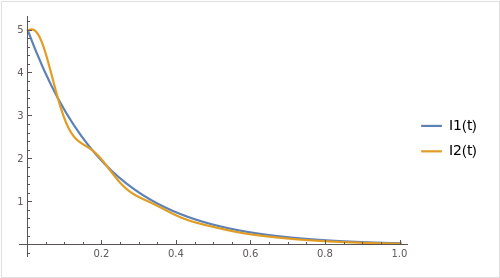
\includegraphics[width=0.75\linewidth]{8c8cda5b-57d1-4cc1-99c2-0a4f0d438c01.png}
        \label{fig:enter-label}
    \end{figure}

    By the graph, the function in question 3 decay to 50\% of initial value after around 0.15 second, while the function in question 6 decay to  50\% of initial value after around 0.13 second.
    

    
\end{solution}

\printbibliography



\end{document}